%%%%%%%%%%%%%%%%%%%%%%%%%%%%%%%%%%%%%%%%%
% Beamer Presentation
% LaTeX Template
% Version 1.0 (10/11/12)
%
% This template has been downloaded from:
% http://www.LaTeXTemplates.com
%
% License:
% CC BY-NC-SA 3.0 (http://creativecommons.org/licenses/by-nc-sa/3.0/)
%
%%%%%%%%%%%%%%%%%%%%%%%%%%%%%%%%%%%%%%%%%

%----------------------------------------------------------------------------------------
%	PACKAGES AND THEMES
%----------------------------------------------------------------------------------------

\documentclass{beamer}

\mode<presentation> {

% The Beamer class comes with a number of default slide themes
% which change the colors and layouts of slides. Below this is a list
% of all the themes, uncomment each in turn to see what they look like.

%\usetheme{default}
%\usetheme{AnnArbor}
%\usetheme{Antibes}
%\usetheme{Bergen}
%\usetheme{Berkeley}
%\usetheme{Berlin}
%\usetheme{Boadilla}
%\usetheme{CambridgeUS}
%\usetheme{Copenhagen}
\usetheme{Darmstadt}
%\usetheme{Dresden}
%\usetheme{Frankfurt}
%\usetheme{Goettingen}
%\usetheme{Hannover}
%\usetheme{Ilmenau}
%\usetheme{JuanLesPins}
%\usetheme{Luebeck}
%\usetheme{Madrid}
%*\usetheme{Malmoe}
%\usetheme{Marburg}
%\usetheme{Montpellier}
%\usetheme{PaloAlto}
%\usetheme{Pittsburgh}
%\usetheme{Rochester}
%\usetheme{Singapore}
%\usetheme{Szeged}
%\usetheme{Warsaw}

% As well as themes, the Beamer class has a number of color themes
% for any slide theme. Uncomment each of these in turn to see how it
% changes the colors of your current slide theme.

%\usecolortheme{albatross}
%\usecolortheme{beaver}
%\usecolortheme{beetle}
%\usecolortheme{crane}
%\usecolortheme{dolphin}
%\usecolortheme{dove}
%\usecolortheme{fly}
%\usecolortheme{lily}
\usecolortheme{orchid}
%\usecolortheme{rose}
%\usecolortheme{seagull}
%\usecolortheme{seahorse}
%\usecolortheme{whale}
%\usecolortheme{wolverine}

%\setbeamertemplate{footline} % To remove the footer line in all slides uncomment this line
%\setbeamertemplate{footline}[page number] % To replace the footer line in all slides with a simple slide count uncomment this line

%\setbeamertemplate{navigation symbols}{} % To remove the navigation symbols from the bottom of all slides uncomment this line
}


\usepackage{graphicx} % Allows including images
\usepackage{booktabs} % Allows the use of \toprule, \midrule and \bottomrule in tables
\usepackage{xspace}
\usepackage{caption}
\usepackage{subfigure}
\usepackage[english,brazil]{babel}
\usepackage[utf8]{inputenc}
\usepackage{listings}
\usepackage{color}

\definecolor{mygreen}{rgb}{0,0.6,0}
\definecolor{mygray}{rgb}{0.5,0.5,0.5}
\definecolor{mymauve}{rgb}{0.58,0,0.82}

%Renomeia o nome padrao das figuras.
\renewcommand{\figurename}{Figura}
\renewcommand{\tablename}{Tabela}



\usepackage[pygopt={texcomments=true,style=emacs}]{pythontex}
\setpythontexlistingenv{listing}

\newcounter{sublisting}[listing]
\newcommand{\codeline}[1]{%
  \addcontentsline{lopytx}{listing}%
    {\protect\numberline{\hspace{0.5in}\thelisting.\arabic{FancyVerbLine}}\hspace{0.5in}#1}%
}


%----------------------------------------------------------------------------------------
%	TITLE PAGE
%----------------------------------------------------------------------------------------

\title[Computação Gráfica]{Espaços de Cores} % The short title appears at the bottom of every slide, the full title is only on the title page

\author{Uéliton Freitas} % Your name
\institute[UFMS] % Your institution as it will appear on the bottom of every slide, may be shorthand to save space
{
Universidade Católica Dom Bosco - UCDB \\ % Your institution for the title page
\medskip
\textit{freitas.ueliton@gmail.com} % Your email address
}
\date{\today} % Date, can be changed to a custom date


\begin{document}

\begin{frame}
\titlepage % Print the title page as the first slide
\end{frame}

\begin{frame}
\frametitle{Sumário} % Table of contents slide, comment this block out to remove it
\tableofcontents % Throughout your presentation, if you choose to use \section{} and \subsection{} commands, these will automatically be printed on this slide as an overview of your presentation
\end{frame}




%----------------------------------------------------------------------------------------
%	PRESENTATION SLIDES
%----------------------------------------------------------------------------------------

%------------------------------------------------
\section{Introdução} 
%------------------------------------------------

%\section{Speeded-Up Robust Features - SURF} % A subsection can be created just before a set of slides with a common theme to further break down your presentation into chunks
%\section{Baf Of Features and Colors}

%\section{Refer\^encias}
%%%%%%%%%%%%%%%%%%%%%%%%%%%%%%%%%%%%%%%%%%%%%%%%%%%%%%%%%%%%%%%%%%%%%%%%%%%%%%%%%%%%%%%%%%
\begin{frame}
\frametitle{Introdução}

		\begin{block}{Espaço de Cores}
			\begin{itemize}
				\item As imagens são obtidas do mundo real representadas de um forma que a mesma pode ser interpretada pelo computador.
				
				\item Há vários métodos de se obter e representar imagens para fins computacionais.
			\end{itemize} 
		\end{block}
		
		\begin{figure}[!h]
			\begin{center}
				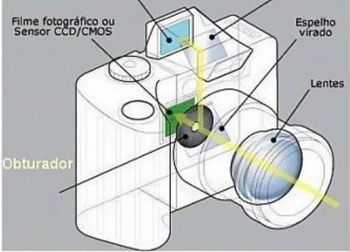
\includegraphics[width=0.4\textwidth]{Figures/cameraDigital}
			\end{center}
		\end{figure}
	
\end{frame}

%%%%%%%%%%%%%%%%%%%%%%%%%%%%%%%%%%%%%%%%%%%%%%%%%%%%%%%%%%%%%%%%%%%%%%%%%%%%%%%%%%%%%%%%%%
\begin{frame}
\frametitle{Introdução}

		\begin{block}{Espaço de Cores}
			\begin{itemize}
				\item As imagens são representadas por meio de matrizes numéricas.
				
				\item Cada posição representa uma intensidade da cor obtida do meio externo.
			\end{itemize} 
		\end{block}
		
		\begin{figure}[!h]
			\begin{center}
				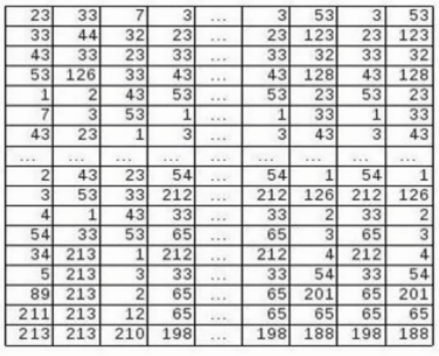
\includegraphics[width=0.4\textwidth]{Figures/table}
			\end{center}
		\end{figure}
	
\end{frame}

%%%%%%%%%%%%%%%%%%%%%%%%%%%%%%%%%%%%%%%%%%%%%%%%%%%%%%%%%%%%%%%%%%%%%%%%%%%%%%%%%%%%%%%%%%
\begin{frame}
\frametitle{Introdução}

		\begin{block}{Espaço de Cores}
			\begin{itemize}
				\item Há vários espaços de cores que podem ser utilizados para representar cores.
			\end{itemize} 
		\end{block}
		
		\begin{figure}[htb!]
  		\centering
   			\subfigure[RGB]{%
     		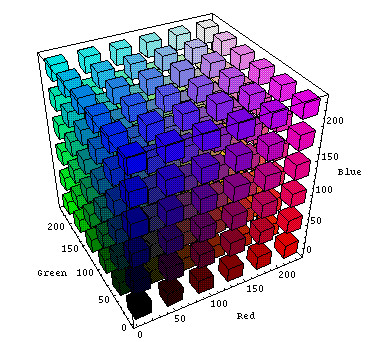
\includegraphics[width=0.2\textwidth]{Figures/RGB}}\qquad
     		\subfigure[CieLab]{%
     		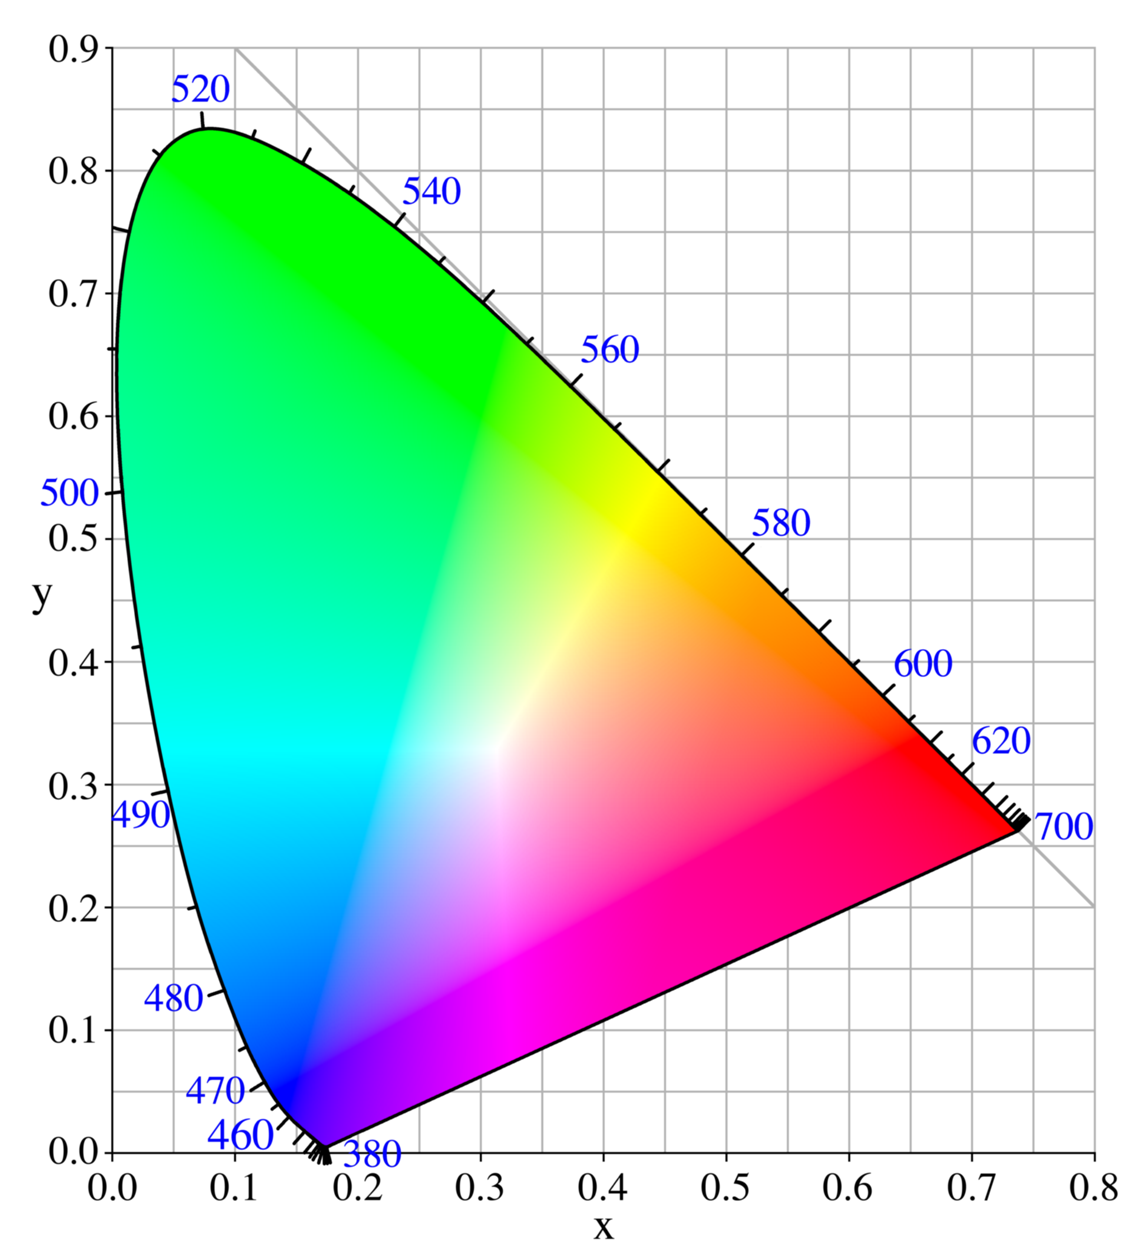
\includegraphics[width=0.2\textwidth]{Figures/CIELAB}}\qquad
     		\subfigure[HSV]{%
     		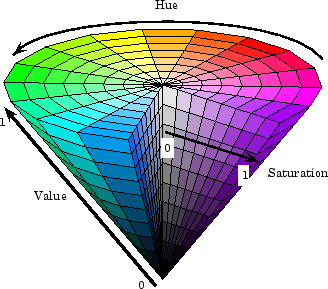
\includegraphics[width=0.2\textwidth]{Figures/HSV}}\qquad
  		\label{iep}
	\end{figure}
	
\end{frame}

\section{RGB - Red, Green e Blue}
%%%%%%%%%%%%%%%%%%%%%%%%%%%%%%%%%%%%%%%%%%%%%%%%%%%%%%%%%%%%%%%%%%%%%%%%%%%%%%%%%%%%%%%%%%
\begin{frame}
\frametitle{RGB}

		\begin{block}{RGB}
			\begin{itemize}
				\item O espaço de cores RGB é um espaço onde a adição de três cores primárias compõem várias outras.
					\begin{itemize}
						\item Red.
						\item Green.
						\item Blue.
					\end{itemize}
			\end{itemize} 
		\end{block}
		
		\begin{figure}[!h]
			\begin{center}
				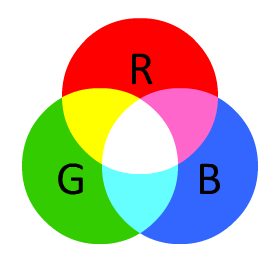
\includegraphics[width=0.3\textwidth]{Figures/PRGB}
			\end{center}
		\end{figure}
	
\end{frame}

%%%%%%%%%%%%%%%%%%%%%%%%%%%%%%%%%%%%%%%%%%%%%%%%%%%%%%%%%%%%%%%%%%%%%%%%%%%%%%%%%%%%%%%%%%
\begin{frame}
\frametitle{RGB}

		\begin{block}{RGB}
			\begin{itemize}
				\item É dependente de dispositivo.
				\item As cores RGB foram escolhidas como sendo primárias devido a fisionomia do olho humano ser melhor estimulado por tais cores, além das mesmas poderem compor qualquer outra cor (há espaços de cores como o CMYK que possui outras cores primárias).
			\end{itemize} 
		\end{block}
		
		\begin{figure}[!h]
			\begin{center}
				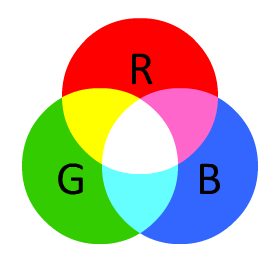
\includegraphics[width=0.3\textwidth]{Figures/PRGB}
			\end{center}
		\end{figure}
	
\end{frame}

%%%%%%%%%%%%%%%%%%%%%%%%%%%%%%%%%%%%%%%%%%%%%%%%%%%%%%%%%%%%%%%%%%%%%%%%%%%%%%%%%%%%%%%%%%
\begin{frame}
\frametitle{RGB}
		
		\begin{figure}[!h]
			\begin{center}
				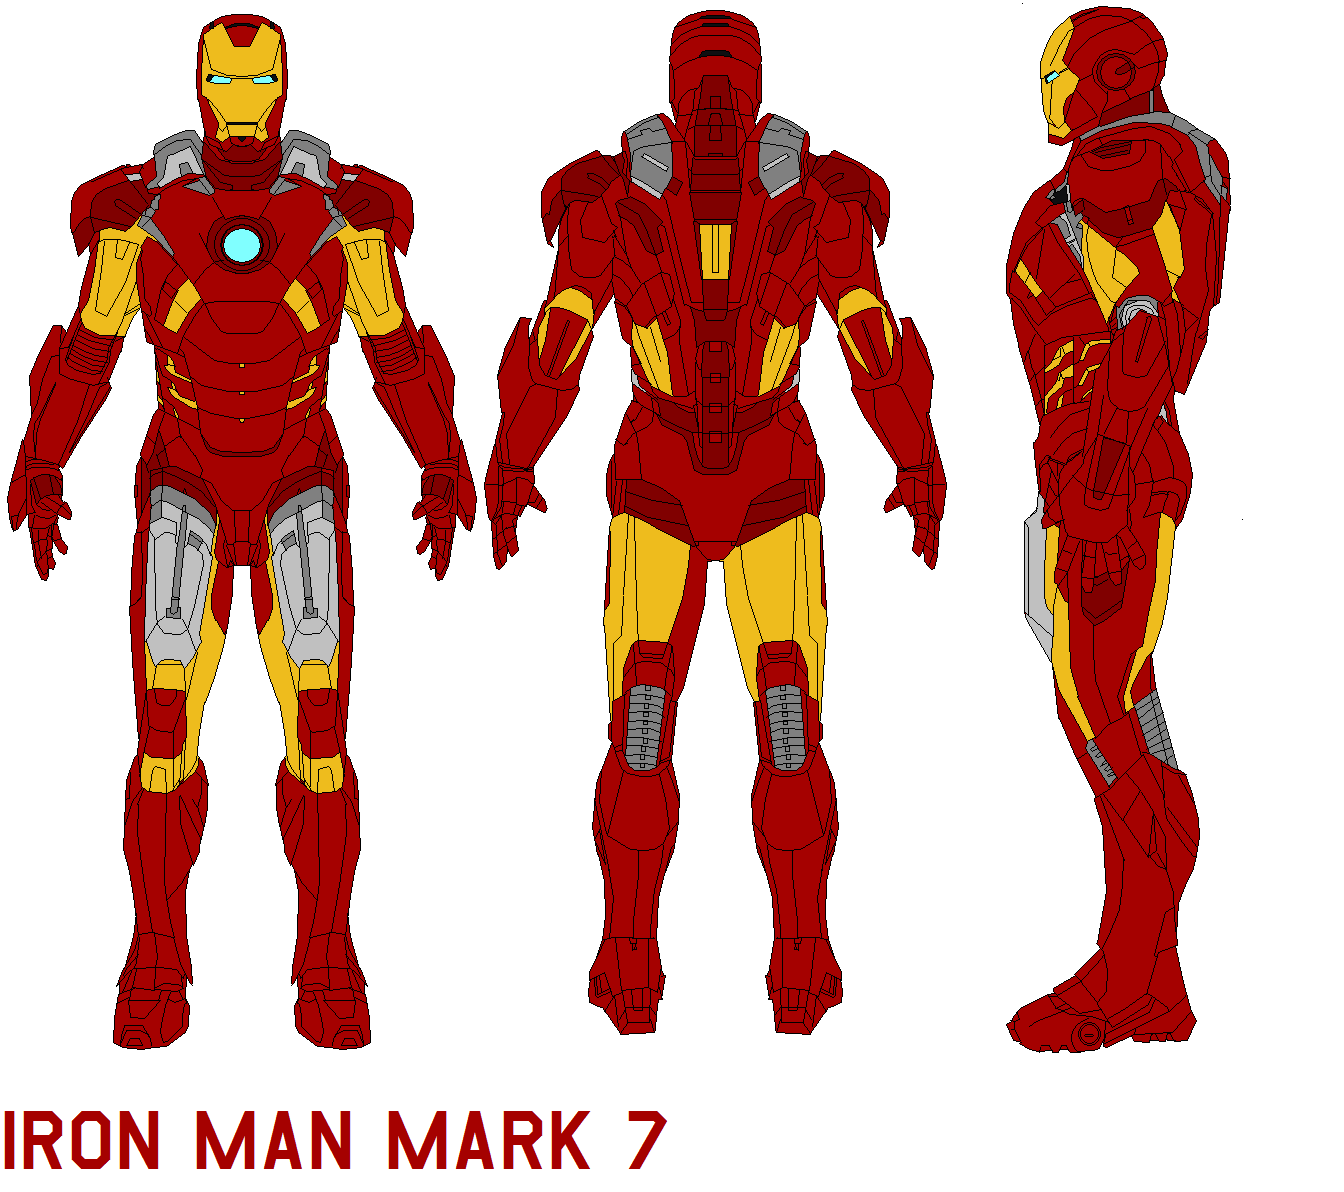
\includegraphics[width=0.7\textwidth]{Figures/Iro}
				\caption{Ironman - RGB.}
			\end{center}
		\end{figure}
	
\end{frame}

%%%%%%%%%%%%%%%%%%%%%%%%%%%%%%%%%%%%%%%%%%%%%%%%%%%%%%%%%%%%%%%%%%%%%%%%%%%%%%%%%%%%%%%%%%
\begin{frame}
\frametitle{RGB}
		
		\begin{figure}[!h]
			\begin{center}
				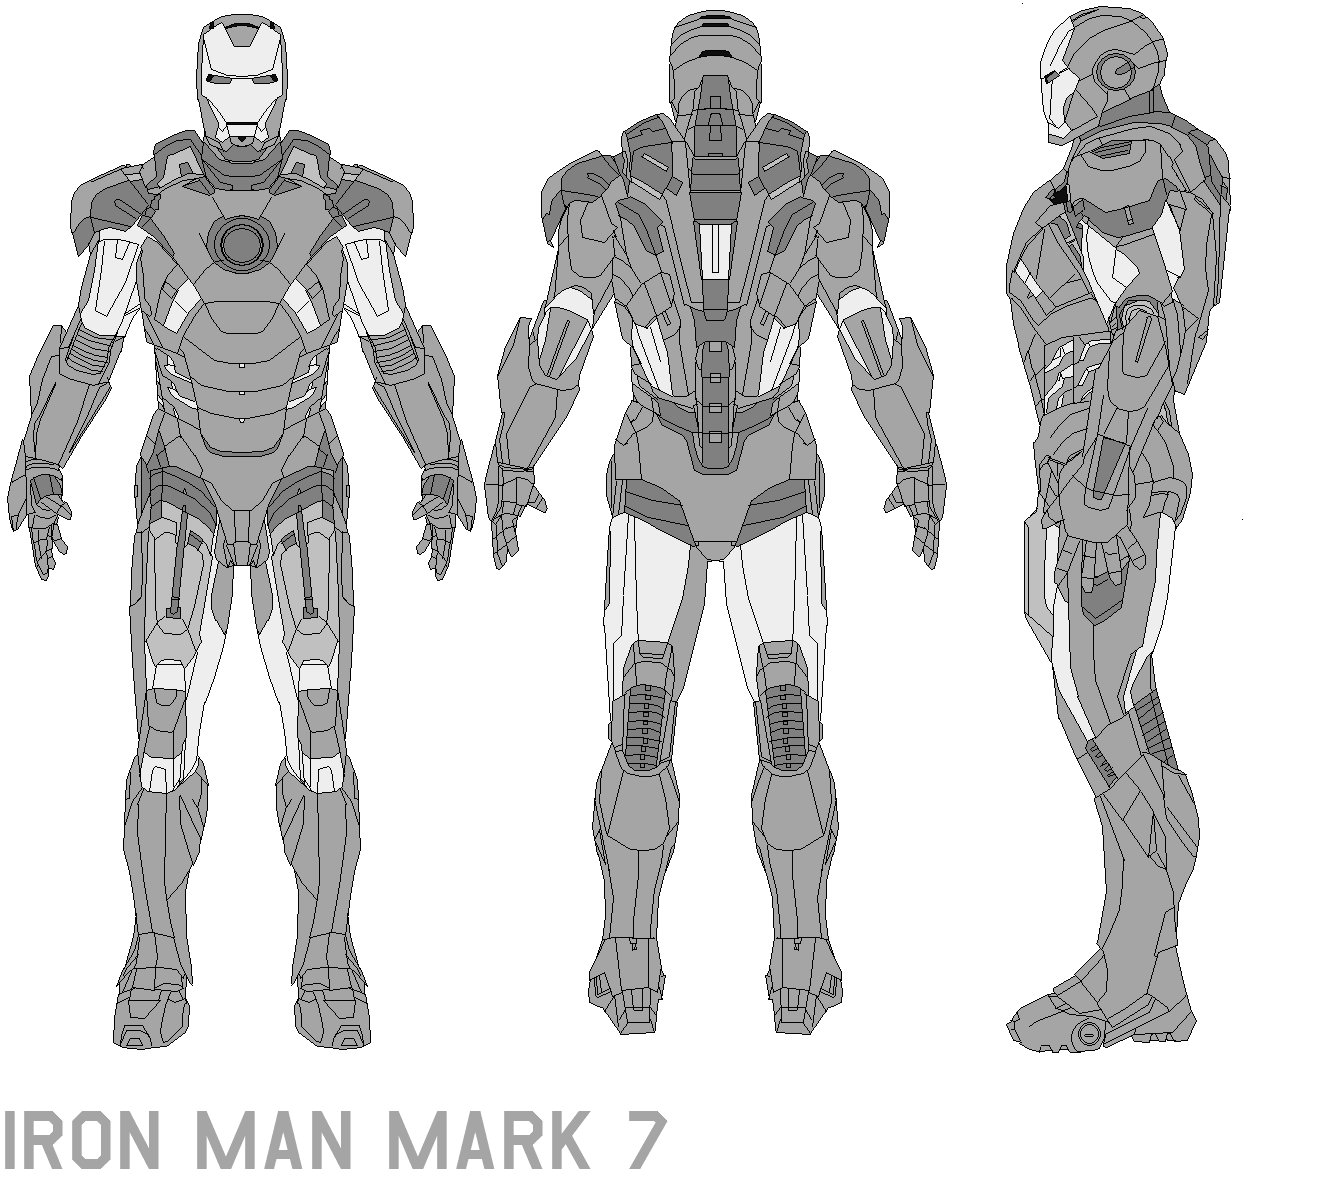
\includegraphics[width=0.7\textwidth]{Figures/Red}
				\caption{Ironman - Red.}
			\end{center}
		\end{figure}
	
\end{frame}

%%%%%%%%%%%%%%%%%%%%%%%%%%%%%%%%%%%%%%%%%%%%%%%%%%%%%%%%%%%%%%%%%%%%%%%%%%%%%%%%%%%%%%%%%%
\begin{frame}
\frametitle{RGB}
		
		\begin{figure}[!h]
			\begin{center}
				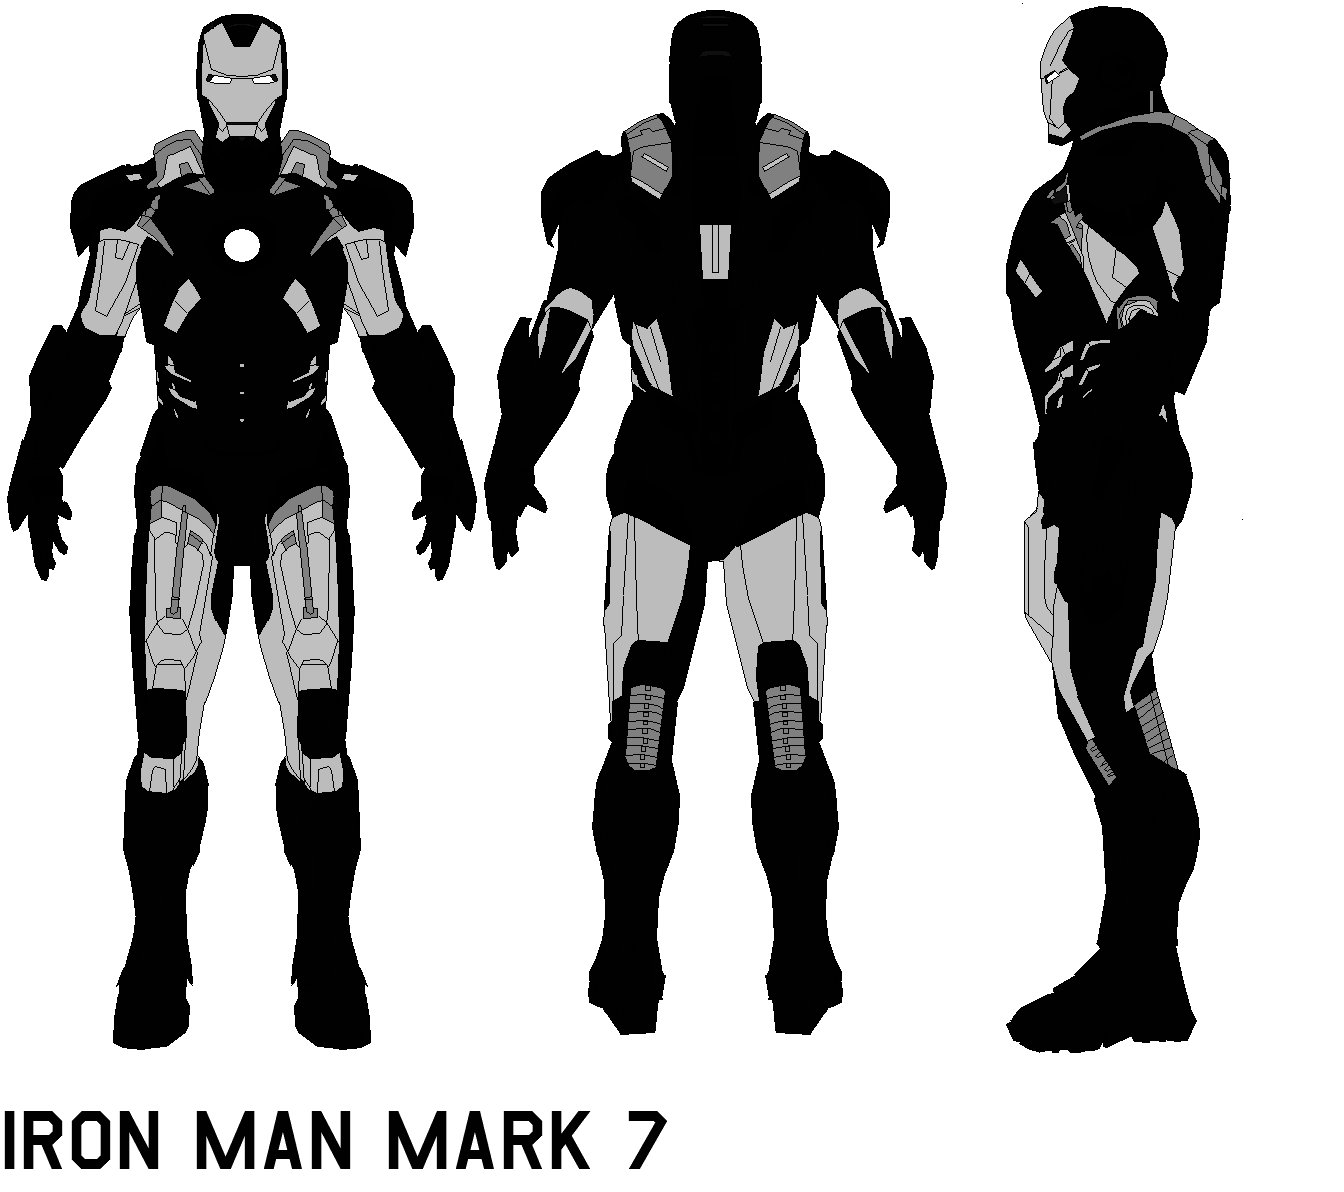
\includegraphics[width=0.7\textwidth]{Figures/Green}
				\caption{Ironman - Green.}
			\end{center}
		\end{figure}
	
\end{frame}

%%%%%%%%%%%%%%%%%%%%%%%%%%%%%%%%%%%%%%%%%%%%%%%%%%%%%%%%%%%%%%%%%%%%%%%%%%%%%%%%%%%%%%%%%%
\begin{frame}
\frametitle{RGB}
		
		\begin{figure}[!h]
			\begin{center}
				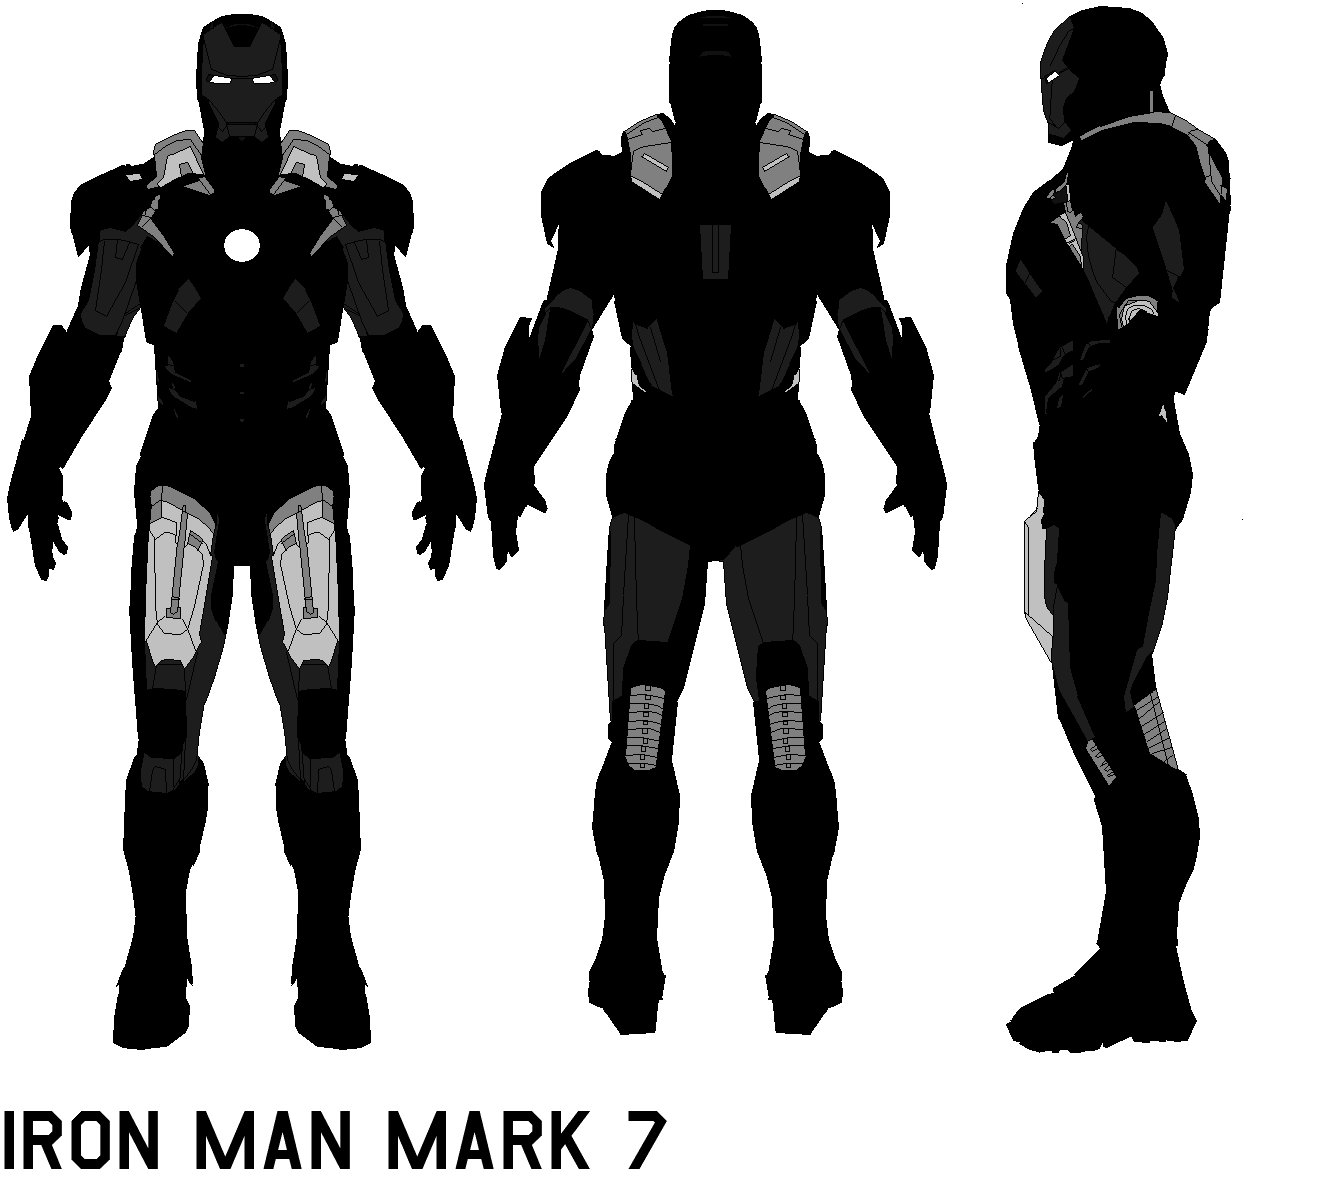
\includegraphics[width=0.7\textwidth]{Figures/Blue}
				\caption{Ironman - Blue.}
			\end{center}
		\end{figure}
	
\end{frame}

\section{HSB - Hue Saturation e Brightness}
%%%%%%%%%%%%%%%%%%%%%%%%%%%%%%%%%%%%%%%%%%%%%%%%%%%%%%%%%%%%%%%%%%%%%%%%%%%%%%%%%%%%%%%%%%
\begin{frame}
\frametitle{HSB}
		
		\begin{block}{HSB}
			\begin{itemize}
				\item O espaço de cores HSB (HSV) é um modo de representar cores, mas de um ``modo'' diferente.
				\begin{itemize}
					\item Hue - Matiz.
					\item Sturation - Saturação.
					\item Brightness - Brilho.
				\end{itemize}
			\end{itemize}
		\end{block}
		
		\begin{figure}[!h]
			\begin{center}
				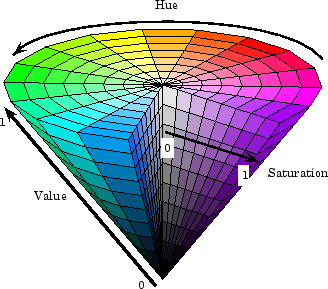
\includegraphics[width=0.4\textwidth]{Figures/HSV}
			\end{center}
		\end{figure}		
\end{frame}


%%%%%%%%%%%%%%%%%%%%%%%%%%%%%%%%%%%%%%%%%%%%%%%%%%%%%%%%%%%%%%%%%%%%%%%%%%%%%%%%%%%%%%%%%%
\begin{frame}
\frametitle{HSB}
		\begin{block}{Motivação}
			\begin{itemize}
				\item Mas por que utilizar o espaço de cores HSB?
			\end{itemize}
		\end{block}
		
		\begin{block}{}
			\begin{itemize}
				\item Seja um dispositivo RGB com a cor laranja.
				\item É desejado uma cor que seja laranja também, mas é desejado que a cor seja menos ``colorida'', ou menos saturada.
			\end{itemize}
		\end{block}
		
		\begin{figure}[!h]
			\begin{center}
				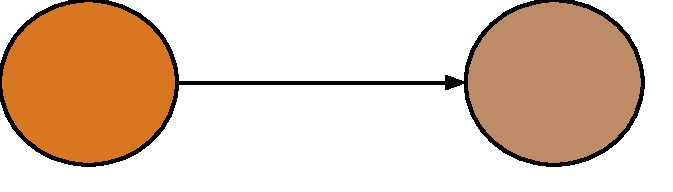
\includegraphics[width=0.6\textwidth]{Figures/Orange}
			\end{center}
		\end{figure}			
	
\end{frame}

		
		%%%%%%%%%%%%%%%%%%%%%%%%%%%%%%%%%%%%%%%%%%%%%%%%%%%%%%%%%%%%%%%%%%%%%%%%%%%%%%%%%%%%%%%%%%
\begin{frame}
\frametitle{HSB}
		\begin{block}{Motivação}
			\begin{itemize}
				\item Para tal fim é necessário variar os valores de R,G e B.
			\end{itemize}
		\end{block}
		
		\begin{figure}[!h]
			\begin{center}
				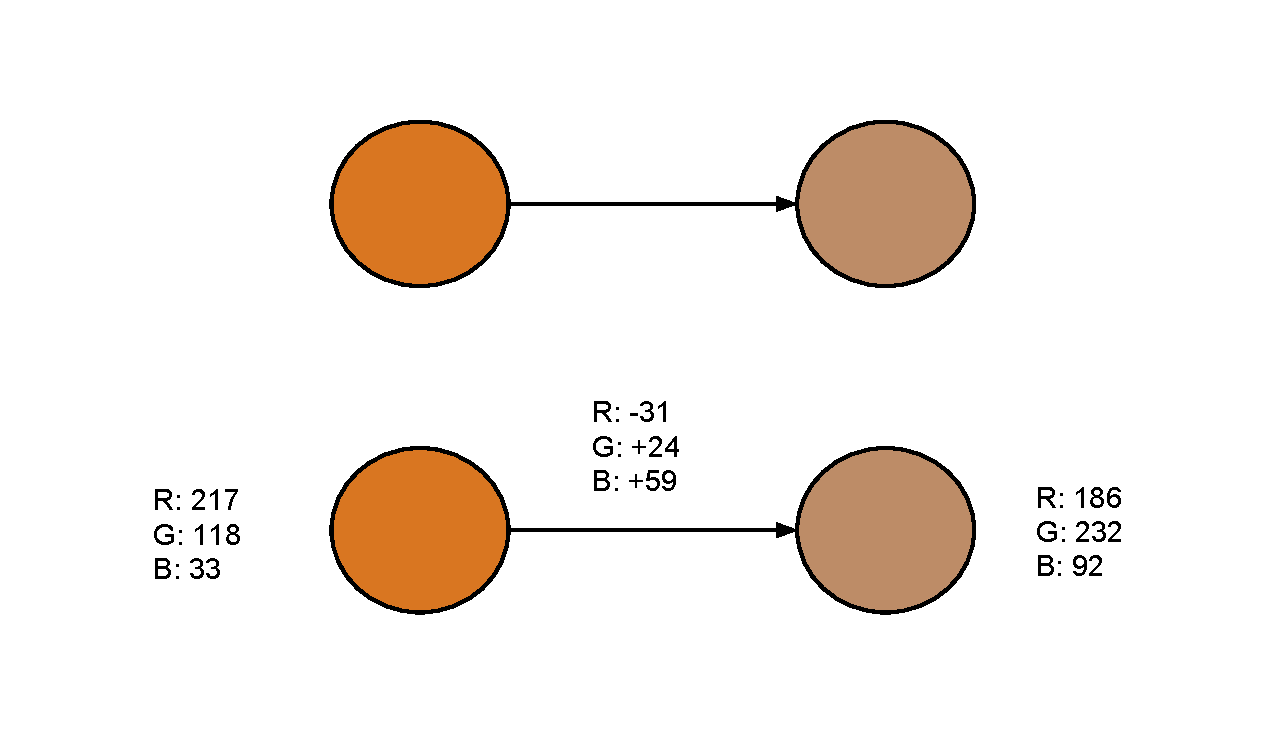
\includegraphics[width=1.0\textwidth]{Figures/WHYHSV}
			\end{center}
		\end{figure}			
\end{frame}

%%%%%%%%%%%%%%%%%%%%%%%%%%%%%%%%%%%%%%%%%%%%%%%%%%%%%%%%%%%%%%%%%%%%%%%%%%%%%%%%%%%%%%%%%%
\begin{frame}
\frametitle{HSB}
		\begin{block}{Motivação}
			\begin{itemize}
				\item Note que não há uma relação entre as variações dos canais R, G e B.
			\end{itemize}
		\end{block}
		
		\begin{block}{}
			\begin{itemize}
				\item Assim, um modelo mais tradicional e intuitivo foi criado para suprir esta necessidade.
				\begin{itemize}
					\item A matiz (Hue) varia a cor.
					\item A saturação varia a ``pureza'' da cor, quanto mais ``viva'' é caro.
					\item O brilho varia de acordo com o brilho da cor, isto é, mais escuro ou não.
				\end{itemize}
			\end{itemize}
		\end{block}		
		
\end{frame}

%%%%%%%%%%%%%%%%%%%%%%%%%%%%%%%%%%%%%%%%%%%%%%%%%%%%%%%%%%%%%%%%%%%%%%%%%%%%%%%%%%%%%%%%%%
\begin{frame}
\frametitle{HSB}
		
		\begin{figure}[!h]
			\begin{center}
				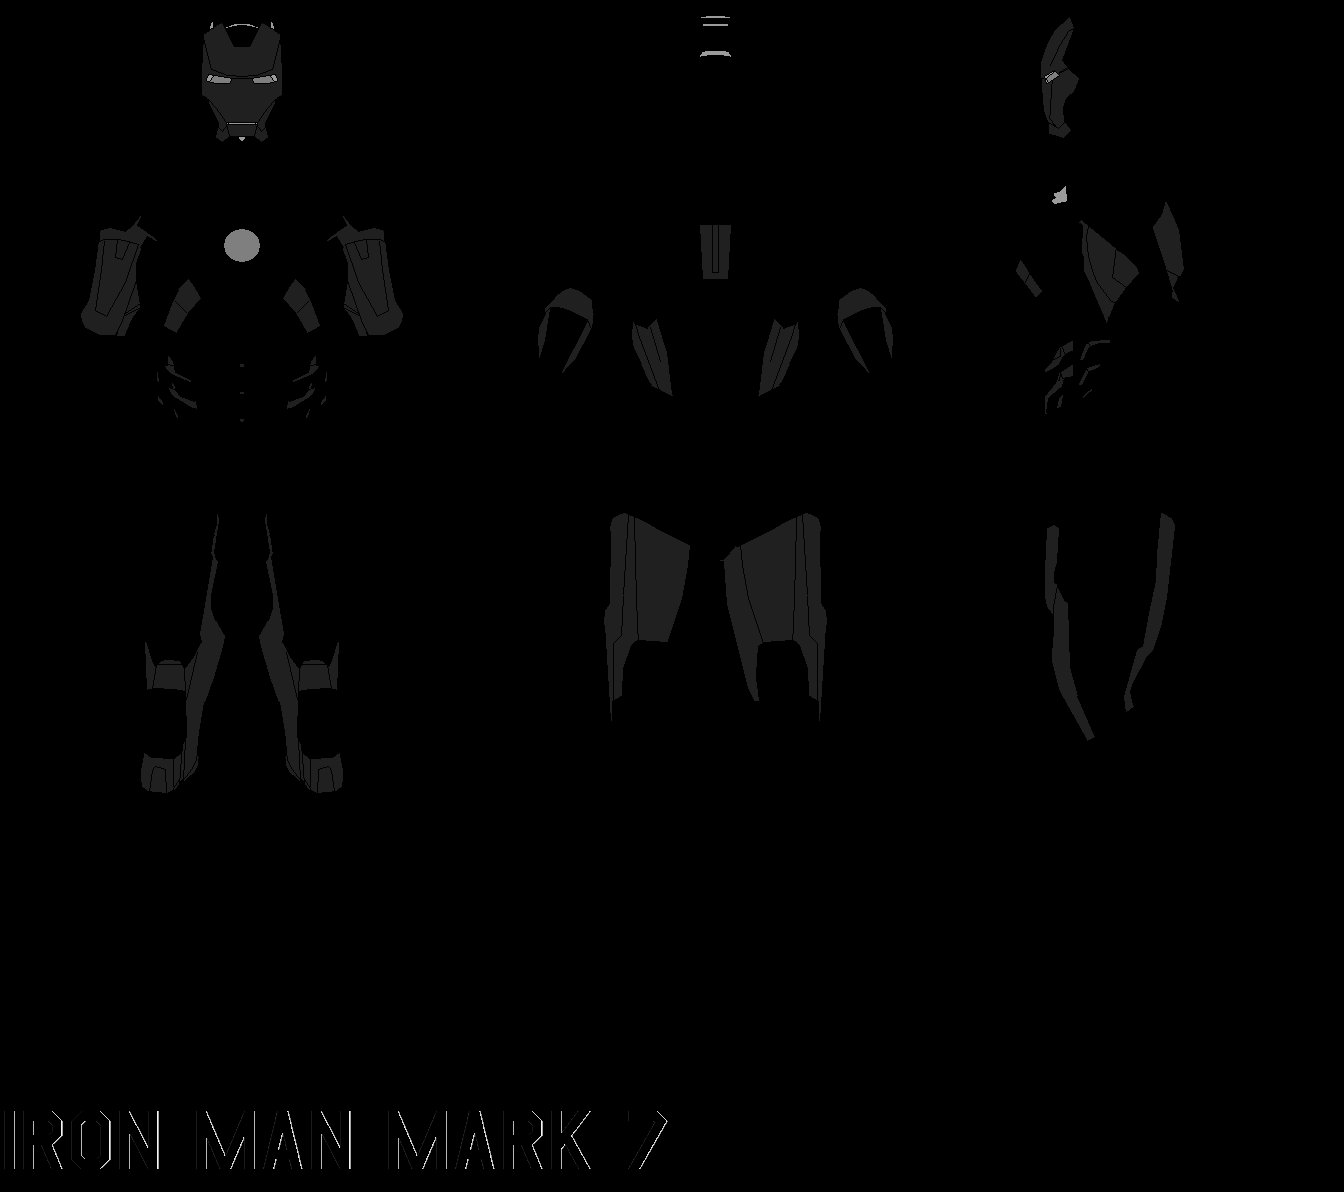
\includegraphics[width=0.7\textwidth]{Figures/Hue}
				\caption{Ironman - Hue.}
			\end{center}
		\end{figure}
	
\end{frame}

%%%%%%%%%%%%%%%%%%%%%%%%%%%%%%%%%%%%%%%%%%%%%%%%%%%%%%%%%%%%%%%%%%%%%%%%%%%%%%%%%%%%%%%%%%
\begin{frame}
\frametitle{HSB}
		
		\begin{figure}[!h]
			\begin{center}
				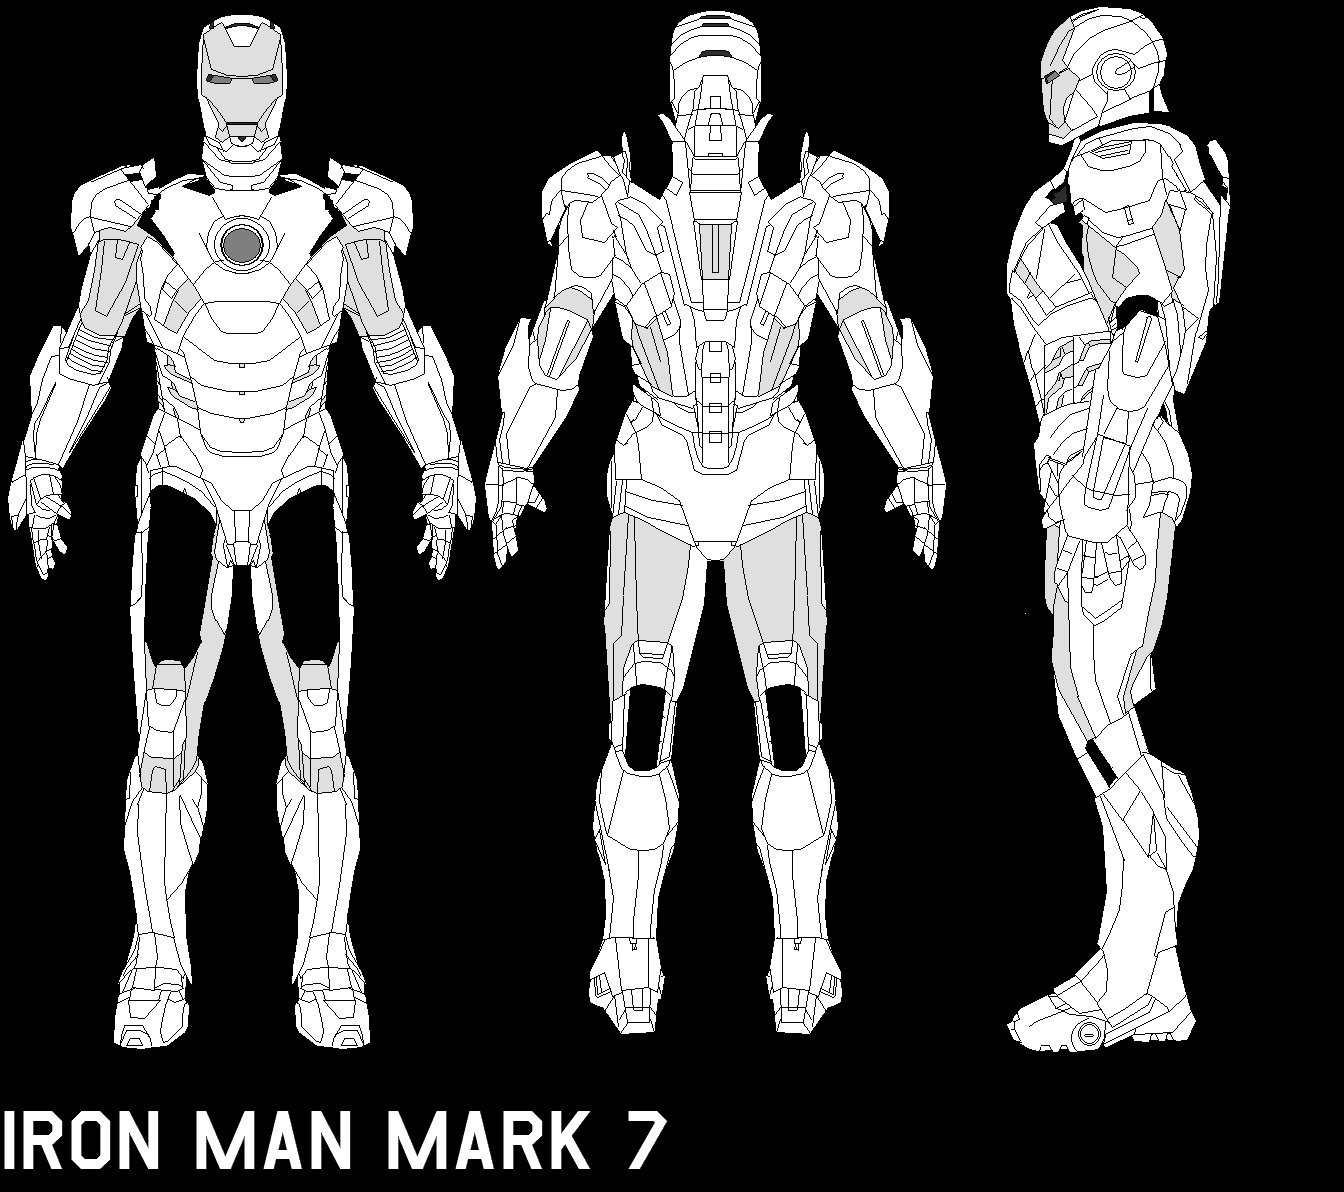
\includegraphics[width=0.7\textwidth]{Figures/Saturation}
				\caption{Ironman - Saturation.}
			\end{center}
		\end{figure}
\end{frame}

%%%%%%%%%%%%%%%%%%%%%%%%%%%%%%%%%%%%%%%%%%%%%%%%%%%%%%%%%%%%%%%%%%%%%%%%%%%%%%%%%%%%%%%%%%
\begin{frame}
\frametitle{HSB}
		
		\begin{figure}[!h]
			\begin{center}
				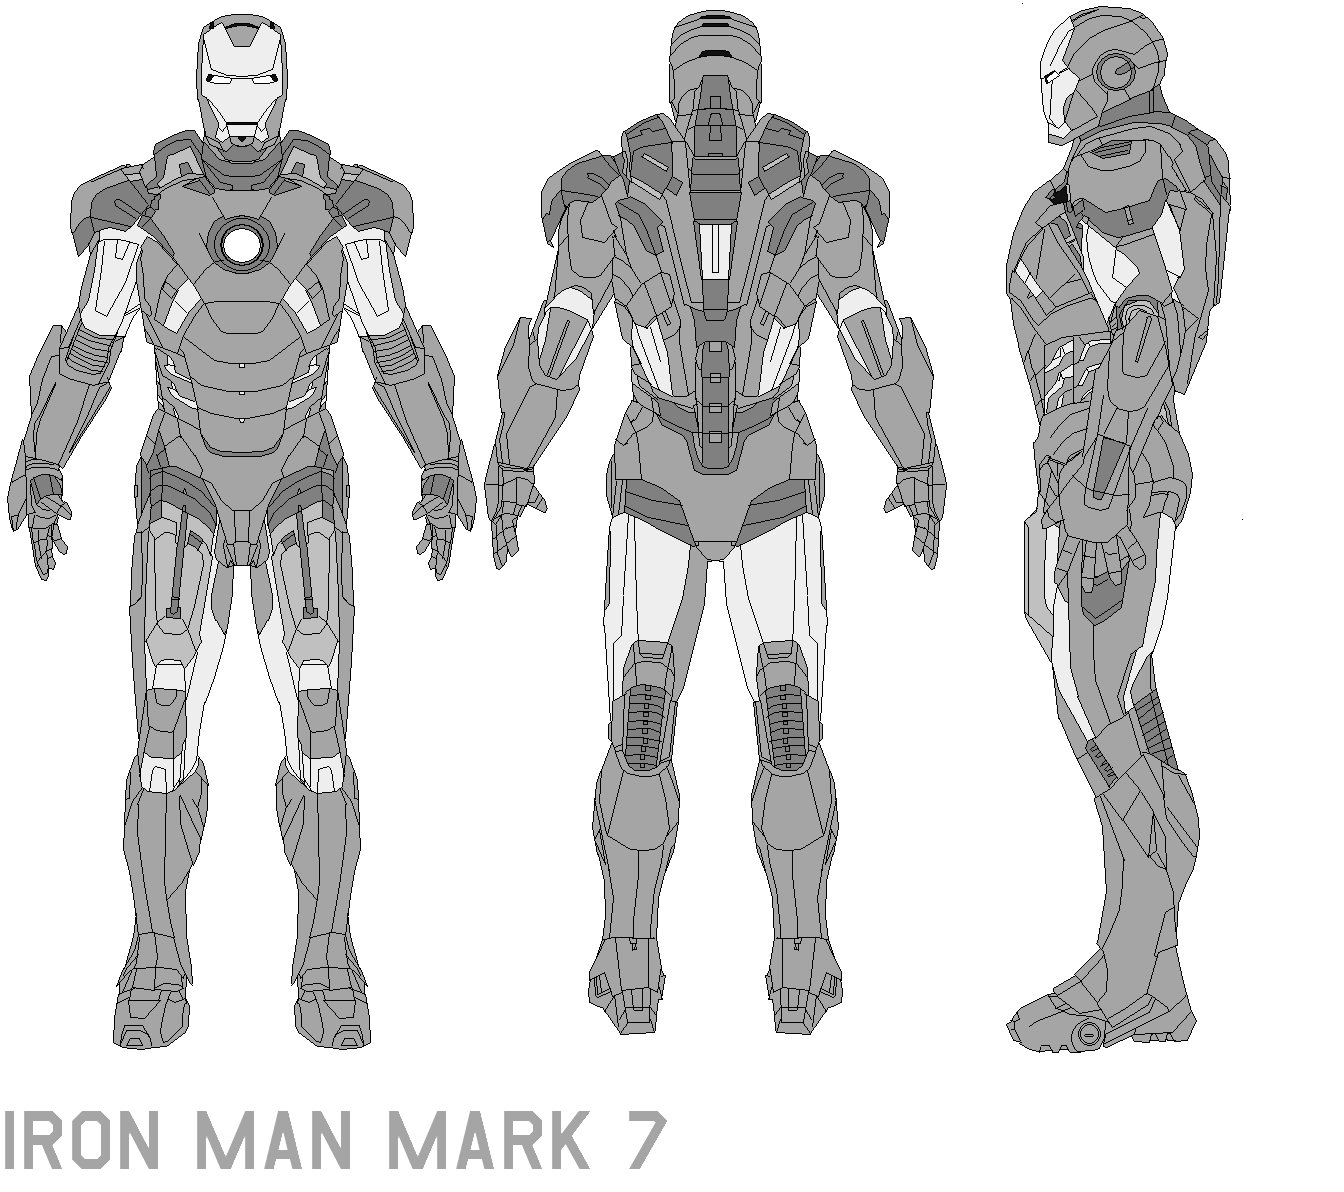
\includegraphics[width=0.7\textwidth]{Figures/Brightness}
				\caption{Ironman - Brightness.}
			\end{center}
		\end{figure}
\end{frame}

%----------------------------------------------------------------------------------------
\end{document} 